\input{../preamble.tex}
\usepackage{minted}

\SetDate[10/03/2026]

\newcommand\calculator{\tikz{
\node (c) [inner sep=0pt, draw, fill=black, anchor=south west]{\phantom{N}};
\begin{scope}[x=(c.south east),y=(c.north west)]
   \fill[white] (.1,.7) rectangle (.9,.9);
   \foreach \x in {.1, .33, .55, .79}{
   \foreach \y in {.1, .24, .38, .53}{
   \fill[white] (\x,\y) rectangle +(.11,.07);}}
\end{scope}
}}


\begin{document}
\pagestyle{fancy}
\fancyhead[L]{Seconde}
\fancyhead[C]{\textbf{Probabilités}}
\fancyhead[R]{\today}

\subsection*{Automatismes}

% why do the solutions not multicols properly?
% really annoying.
%\begin{multicols}{2}
\exe{}{
	On lance une pièce de monnaie bien équilibrée.
	\begin{enumerate}
		\item Décrire les issues de l'expérience.
		\item Après 10 000 lancers, combien de fois « pile » peut-on s'attendre à avoir eu ?
		\item Donner la probabilité de chaque issue.
	\end{enumerate}
}{exe:aut1}{
	\begin{enumerate}
		\item 
		Les deux issues sont « pile » et « face ».
		En mathématiques, obtenir la tranche n'est pas possible !
		\item 
		La pièce étant bien équilibrée : on s'attend donc à obtenir 5 000 fois « pile » et 5 000 fois « face ».
		\item
		La probabilité d'obtenir « pile » est $\frac12$ et celle d'obtenir $\frac12$.
		On peut, pour donner une intuition aux probabilités, les voir comme un fréquence ($\frac{5~000}{10~000} = \frac12$).
		À terme, il faudra cependant voir la probabilité comme un modèle mathématique fixé : la fréquence s'approche de la probabilité lorsqu'on multiplie les expériences, et non pas l'inverse !
	\end{enumerate}
	
}

%\columnbreak

\exe{}{
	On lance un D6 équilibré, dé à 6 faces, puis on lit le numéro de la face du dessus.
	\begin{enumerate}
		\item Décrire les issues de l'expérience.
		\item Après 60 000 lancers, combien de 6 peut-on s'attendre à avoir eu ?
		%\item Donner la probabilité de chaque issue.
		\item Donner la probabilité d'obtenir un nombre pair.
		%\item Donner la probabilité d'obtenir un multiple de $3$.
	\end{enumerate}
}{exe:aut2}{
	\begin{enumerate}
		\item 
		Les issues sont « 1 », « 2 », « 3 », « 4 », « 5 », et « 6 ».
		\item 
		Comme le dé est bien équilibré, on peut s'attendre à obtenir 10 000 fois 6.
%		\item 
%		Comme le dé est bien équilibré, leur probabilité est $\frac16$.
%		À nouveau, la probabilité est liée à la fréquence dans un sens uniquement : la probabilité est admise, et la fréquence s'approche de celle-ci lorsque le nombre de lancers devient grand.
		\item 
		Trois issues correspondent à l'événement « obtenir un nombre pair » et on ajoute leur probabilité : $\frac16 + \frac16 + \frac16 = \frac12$.
	\end{enumerate}
}
%\end{multicols}

%\vspace{-10pt}

\exe{}{
	Une urne contient 3 boules rouges, 2 boules noires, et 5 boules vertes. On tire une boule au hasard et on note sa couleur.
	\begin{enumerate}
		\item Décrire les issues de l'expérience.
		\item Après $50~000$ tirages avec remise, combien de boules noires peut-on s'attendre à avoir tiré ?
		\item Donner la probabilité de chaque issue.
	\end{enumerate}
}{exe:aut3}{
	\begin{enumerate}
		\item
		Les troies issues sont « Rouge », « Noir », et « Vert ».
		\item 
		Comme 2 dizième des boules sont rouges, on s'attend à avoir tiré 
			\[ 50~000\times\frac2{10} = 10~000 \]
		fois « Noir ».
		De façon similaire, on s'attend à avoir tiré 15 000 fois « Rouge » et 25 000 fois « Vert ».
		\item 
		La probabilité d'obtenir « Rouge » est $\frac3{10}$, la probabilité d'obtenir « Noir » est $\frac2{10}$, et la probabilité d'obtenir « Vert » est $\frac5{10}$.
		La fraction peuvent être simplifiées si voulu.
		Remarquons que leur somme vaut $\frac3{10}+\frac2{10}+\frac5{10} = 1$.
	\end{enumerate}
}

\exe{}{
	Donner les ensembles résultant de l'union et de l'intersection.
	\begin{multicols}{2}
	\begin{enumerate}
		\item $\bigset{ 1 ; 2 ; -2 ; -4 } \cap \bigset{  -1; 2 ; -4 ; 1 }$
		\item $\bigset{ 1 ; 2 ; -2 ; -4 } \cup \bigset{  -1; 2 ; -4 ; 1 }$
	\end{enumerate}
	\end{multicols}
}{exe:inter-union}{
	\begin{multicols}{2}
	\begin{enumerate}
		\item $\bigset{ 1 ; 2 ; -4 }$
		\item $\bigset{1;2;-2;-4;-1;1}$
	\end{enumerate}
	\end{multicols}
}

%\vspace{-10pt}
\subsection*{Exercices}


%\exe{}{
%	Donner l'univers $\Omega$ de chacune des expériences aléatoires suivantes.
%	\begin{multicols}{2}
%	\begin{enumerate}[label=---]
%		\item Un lancer de dé équilibré à six faces.
%		\item Un lancer de dé pipé (truqué) à six faces.
%		\item Un lancer de pièce de monnaie.
%		\item Deux lancers de dés  à $6$ faces simultanés.
%		\item Deux lancers de dés à $6$ faces, l'un après l'autre.
%		\item Couleur d'une carte tirée au hasard parmis un jeu de $52$ cartes.
%	\end{enumerate}
%	\end{multicols}
%}{exe:exe00}{
%
%	\begin{multicols}{2}
%	\begin{enumerate}
%		\item $\Omega = \{ 1 ; 2 ; 3 ;4 ;5 ;6\}$.
%		\item $\Omega = \{ 1 ; 2 ; 3 ;4 ;5 ;6\}$.
%		\item $\Omega = \{ \text{Pile} ; \text{Face} \}$.
%		\item $\Omega = \left\{ \{a ; b \} \text{ où } a, b \in \{ 1 ; 2 ; 3 ;4 ;5 ;6\} \right\}$.
%		\item $\Omega = \left\{ ( a ;b ) \text{ où } a, b \in \{ 1 ; 2 ; 3 ;4 ;5 ;6\} \right\}$.
%		\item $\Omega = \{ \text{Carreau} ; \text{Cœur} ; \text{Trèfle} ; \text{Pique} \}$.
%	\end{enumerate}
%	\end{multicols}
%
%
%}

\exe{}{
	On lance un D20, dé à 20 faces numérotées de $1$ à $20$.
	On note le nombre de la face du dessus.
	\begin{enumerate}
		\item Donner l'univers $\Omega$ ainsi que son cardinal $|\Omega|$.
		\item Pour chacun des événements suivants, donner l'ensemble des issues associé ainsi que son cardinal.
			\begin{multicols}{2}
			\begin{enumerate}[label=\roman*)]
			\item A : « le nombre est pair »
			\item B : « le nombre est multiple de $3$ »
			\columnbreak
			\item C : \mbox{« le nombre est multiple de $3$ \textbf{ou} pair »}
			\item D : \mbox{« le nombre est multiple de 3 \textbf{et} pair »}
			\end{enumerate}
			\end{multicols}
		\item
		Peut-on connaitre la probabilité de chacun de ces événements ?
	\end{enumerate}
}{exe:univers2}{
	\begin{enumerate}
		\item $\Omega = \bigset{ 1 ; 2 ; \dots ; 19 ; 20 } = \bigset{ i \in \N \tq 1 \leq i \leq 20 }$ de cardinal $|\Omega| = 20$.
		\item 
		Notons $a | b$ la relation « $a$ divise $b$ ».
		%\begin{multicols}{2}
		\begin{enumerate}[label=\roman*)]
		\item $A = \bigset{ 2 ; 4 ; \dots ; 18 ; 20 } = \bigset{ i \in \N \tq 1 \leq i \leq 20 \et 2|i }$ de cardinal $|A| = 10$
		\item $B = \bigset{ 3 ; 6 ; \dots ; 15 ; 18 } = \bigset{ i \in \N \tq 1 \leq i \leq 20 \et 3|i }$ de cardinal $|B| = 6$
		\item $C = A \cup B = \bigset{ 2 ; 3 ; 4 ; 6 ; 8 ; 9 ; 10 ; 12 ; 14 ; 15 ; 16 ; 18 ; 20 }$ de cardinal $|C| = 13$
		\item $D = A \cap B = \bigset{ 6 ; 12 ; 18 }$ de cardinal $|D| = 3$.
		\end{enumerate}
		%\end{multicols}
		
	\item
	Non, il n'est pas possible de calculer la probabilité de chaque événement sans hypothèse en plus sur le dé.
	En effet, le dé pourrait être bien équilibré (c'est le cas dans l'exercice \ref{exe:D20}), mais il pourrait tout aussi bien être lesté, biaisant le lancer vers l'une ou l'autre face.
	Comme ceci change les probabilités, on ne peut \emph{a priori} rien dire sur celles-ci pour l'instant.
	\end{enumerate}
}


\exe{}{
	On suppose désormais le D20 de l'exercice \ref{exe:univers2} bien équilibré.
	\begin{enumerate}
		\item 
		Calculer la probabilité de chacun des événements de l'exercice \ref{exe:univers2}.
		%\item Vérifier que $D = A \cup B$.
		%\item Vérifier que $E = A \cap B$.
		\item 
		L'égalité suivante est-elle vraie ?
			\[ P(A \cup B) \stackrel{?}{=} P(A) + P(B) - P(A\cap B). \]
	\end{enumerate}
}{exe:D20}{
	\begin{enumerate}
		\item 
		Comme le dé est bien équilibré, chaque issue admet la même probabilité, soit $\frac1{\Omega} = \frac1{20}$.
		En outre, d'après le cours, pour un événement $V = \{ e_1 ; e_2 ; \dots \} \subset \Omega$, sa probabilité est la somme des probabilités des issues lui appartenant.
		C'est donc 
			\[ P(V) = \frac{|V|}{|\Omega|} = \frac{|V|}{20}, \]
		résultat qu'on applique aux quatre événements de l'exercice \ref{exe:univers2} pour trouver
			\begin{align*}
				P(A) &= \frac{10}{20} = \frac12 & P(B) &= \frac{6}{20} = \frac3{10} \\ %&& P(C) = \frac15 \\
				P(C) &= \frac{13}{20} & P(D) &= \frac{3}{20}  % && P(F) = \frac{3}{20}
			\end{align*}
		%\item On vérifie que $D = A \cup B$ en considérant tous les éléments qui appartiennent à $A$ \textbf{ou} à $B$ (ou inclusif : un élément qui appartient aux deux ensembles appartient à l'union) et en vérifiant qu'on trouve bien $D$.
		%\item On vérifie que $E = A \cap B$ en considérant tous les éléments qui appartiennent à $A$ \textbf{et} à $B$ et en vérifiant qu'on trouve bien $E$.
		\item 
		Le membre de gauche de l'identité donne
			\[ P (A \cup B) = P(C) = \frac{13}{20}, \]
		d'après les questions précédentes.
		Le membre de droite de l'identité est égal à 
			\[ P(A) + P(B) - P(A\cap B) = P(A) + P(B) - P(D) = \frac{10}{20} + \frac{6}{20}  - \frac{3}{20} = \frac{13}{20}.\]
		L'identité est donc bien vérifée dans ce cas !
	\end{enumerate}
}

\newpage

\exe{}{
	Compléter le tableau de probabilités concernant le numéro de la face du dessus obtenue après un lancer d'un D6 pipé puis 
	calculer les probabilités suivantes.
	\begin{center}
	\begin{tabular}{|c|c|c|c|c|c|c|} \hline
		Résultat & 1 & 2 & 3 & 4 & 5 & 6 \\ \hline
		Probabilité & $0,1$ & $0,2$ & $0,1$ & $0,15$ & $0,25$ & \\ \hline
	\end{tabular}
	\end{center}
	
	\begin{multicols}{2}
	\begin{enumerate}[label=\roman*)]
		\item P(« obtenir un nombre pair ») 
		\item P(« obtenir un nombre impair ») 
		%\item P(« obtenir un nombre pair »)   + P(« obtenir un nombre impair ») 
		\item P(« obtenir $2$ ou $5$ ») 
		\item P(« obtenir ni $2$ ni $5$ ») 
		%\item P(« obtenir $2$ ou $5$ »)  + P(« obtenir ni $2$ ni $5$ ») 
	\end{enumerate}
	\end{multicols}
}{exe:D6-pipé}{
	On complète d'abord le tableau en sachant que l'univers de l'expérience est $\Omega = \bigset{ 1 ; 2 ;3 ; 4 ; 5 ; 6 }$ et que la somme des probabilités du tableau est donc nécessairement $1$.
	En effet, $P(\Omega) = 1$, car $\Omega$ correspond à l'événement « obtenir une des issues », qui est un événement sûr.
	
	
	\begin{center}
	\begin{tabular}{|c|c|c|c|c|c|c|} \hline
		Résultat & 1 & 2 & 3 & 4 & 5 & 6 \\ \hline
		Probabilité & $0,1$ & $0,2$ & $0,1$ & $0,15$ & $0,25$ & $\color{RED_E} 0,2$ \\ \hline
	\end{tabular}
	\end{center}

	\begin{enumerate}[label=\roman*)]
		\item P(« obtenir un nombre pair ») $ = P(2) + P(4) + P(6) = 0,2 + 0,15 + 0,2 = 0,55$
		\item P(« obtenir un nombre impair ») $ = P(1) + P(3) + P(5) = 0,1 + 0,1 + 0,25 = 0,45$.
		%\item P(« obtenir un nombre pair »)   + P(« obtenir un nombre impair ») $ = 0,55 + 0,45 = 1$
		\item P(« obtenir $2$ ou $5$ ») $ = P(2) + P(5) = 0,2 + 0,25 = 0,45$
		\item P(« obtenir ni $2$ ni $5$ ») $ = P(1) + P(3) + P(4) + P(6) = 0,1 + 0,1 + 0,15 + 0,2 = 0,55$
		%\item P(« obtenir $2$ ou $5$ »)  + P(« obtenir ni $2$ ni $5$ ») $ = 0,45 + 0,55 = 1$
	\end{enumerate}
	
	Le fait que la somme soit $1$ n'est pas suprenant : les événements comptent séparément toutes les issues.
	On appelle ces événements \emph{complémentaires} : ils sont disjoints (les deux événements ne peuvent pas arriver en même temps), et ensembles ils forment l'univers tout entier (chaque issue appartient à un événement ou à l'autre).
	
	Les derniers événements motivent la relation 
		\[ \overline{A \cup B} = \overline{A} \cap \overline{B} \]
	qui, avec des mots, dit
		\begin{center}
			« non (A ou B) » $=$ « ni A, ni B » $=$ « (non A) et (non B) ».
		\end{center}
}




\exe{}{
	Une joueuse de tennis a une probabilité $0,58$ de réussir son premier service et une probabilité de $0,06$ de faire une double faute.
	Quelle est la probabilité qu'elle réussisse son deuxième service ?
}{exe:exe6}{
 	Les issues du service sont $\Omega = \{ \text{Premier service réussi} ; \text{Premier service raté, deuxième réussi} ; \text{Premier et deuxième services ratés} \}$.
	 La somme des probabilité vaut $1$ ($P(\Omega) = 1$), et donc on a nécessairement
	 	\[ P(\text{Premier service raté, deuxième réussi}) = 1 - 0,58 - 0,06 = 0,36. \]
}

\exe{, difficulty=1}{
	On lance un D300 bien équilibré, dé à 300 faces numérotées de 1 à 300.
	Après le lancer, on note le numéro de la face supérieure.
	Posons $A$ : « le résultat n'est pas multiple de 10 », et $B$ : « le résultat n'est pas divisible par 7 ».
	
	\begin{enumerate}
		\item Décrire avec des mots les événements suivants.
			\begin{multicols}{4}
			\begin{enumerate}[label=\roman*)]
				\item $\overline{A}$
				\item $\overline{B}$
				\item $\overline{A} \cap \overline{B}$
				\item $\overline{A} \cup \overline{B}$
				%\item $\overline{A \cup B}$
				%\item $\overline{A \cap B}$
			\end{enumerate}
			\end{multicols}
		\item Calculer les probabilités $P\bigl( \overline{A} \bigr)$ et $P\bigl( \overline{B} \bigr)$.
		\item Justifier à l'aide de sa décomposition en facteurs premiers qu'un multiple à la fois de 7 et de 10 est un multiple de 70.
		\item En déduire $P\bigl(\overline{A} \cap \overline{B}\bigr)$. %étant donné qu'un multiple à la fois de 7 et de 10 est un multiple de 70.
		\item Énoncer le principe d'inclusion-exclusion puis l'utiliser pour calculer $P\bigl(\overline{A} \cup \overline{B}\bigr)$.
		%\item Calculer la probabilité que le résultat obtenu soit supérieur ou égal à $10$.
		\item
		Combien d'entiers entre 1 et 300 sont multiples de 7 ou de 10 ?
	\end{enumerate}
}{exe:D300}{
	\begin{enumerate}
		\item 
			\begin{enumerate}[label=\roman*)]
				\item $\overline{A}$ : « le résultat est multiple de $10$ »
				\item $\overline{B}$ : « le résultat est divisible par $7$ »
				\item $\overline{A} \cap \overline{B}$  : « le résultat est multiple de $10$ \textbf{et} divisible par $7$ »
				\item $\overline{A} \cup \overline{B}$ : « le résultat est multiple de $10$ \textbf{ou} divisible par $7$ »
			\end{enumerate}
		\item 
		Le dé étant bien équilibré, nous sommes en situation d'équiprobabilité et 
			\[ P(E) = \frac{|E|}{|\Omega|} = \frac{|E|}{300} \]
		pour n'importe quel événement $E\subseteq\Omega$.
		Il s'agit donc de calculer le cardinal de $\overline{A}$ et de $\overline{B}$, c'est-à-dire le nombre d'entiers entre $1$ et $300$ qui sont multiples de $10$ puis qui sont multiples de $7$.
		
		D'une part, les multiples de $10$ s'écrivent
			\begin{align*}
				10 \times 1 && 10 \times 2 && 10 \times 3 && \dots && 10 \times 30 = 300,
			\end{align*}
		et donc $|\overline{A}| = 30$, et $P\left( \overline{A} \right) = \frac{30}{300} = \frac1{10}$.
		
		D'autre part, les multiples de $7$ s'écrivent
			\begin{align*}
				7 \times 1 && 7\times 2 && 7 \times 3 && \dots
			\end{align*}
		Pour savoir jusqu'où aller, on calcule $\frac{300}{7} \approx 42,86$, donc la liste s'arrête à $7 \times 42 = 294$.
		Par conséquent, $|\overline{B}| = 42$, et $P\left( \overline{B} \right) = \frac{42}{300} = \frac{7}{50}$ (pas exactement un septième, donc !).
		
		\item
		Soit $n\in\N$ ($n\neq0$) un multiple à la fois de 7 et de 10.
		Comme $n$ est divisible par 7, il admet au moins un 7 dans un sa décomposition en facteurs premiers.
		Comme $n$ est divisble par $10 = 2 \times 5$, il admet au moins un 2 et au moins un 5 dans sa décomposition en facteurs premiers.
		Ainsi, $n$ doit s'écrire $n = 7\times2\times5\times k$, avec $k\in\N$ le reste de la décomposition.
		D'où $n = 70\times k$, avec $k$ entier : $n$ est multiple de 70.
		
		\item 
		Calculons d'abord $P\bigl(\overline{A} \cap \overline{B}\bigr)$ en comptant les multiples de 70 supérieurs ou égaux à 1 et inférieurs ou égaux à $300$.
		Ceux-ci sont $\bigset{ 70 ; 140 ; 210 ; 280 }$.
		D'où $P\bigl(\overline{A} \cap \overline{B}\bigr) = \frac{4}{300} = \frac{1}{75}$.
		
		\item
		Utilisons l'inclusion-exclusion pour conclure :
			\begin{align*}
				P\bigl(\overline{A} \cup \overline{B}\bigr) &= P\bigl( \overline{A} \bigr) + P\bigl( \overline{B} \bigr) - P\bigl(\overline{A} \cap \overline{B}\bigr) \\
																&= \frac{30}{300} + \frac{42}{300} -  \frac{4}{300} \\
																&= \frac{68}{300} = \frac{17}{75}.
			\end{align*}
		
		\item
		Remarquons qu'on a ainsi compté le nombre d'entier entre 1 et 300 qui sont multiples de 7 ou de 10 : il y en a 68.

%		\item 
%		L'événement correspond à l'ensemble 
%			\[ \{10 ; 11 ; 12 ; \dots ; 299 ; 300 \}, \]
%		de cardinal $300-10+1 = 291$ (pour se convaincre de la nécessité du $+1$, essayer de calculer le cardinal de $\{10 ; 11\}$, puis $\{10 ; 11 ; 12 \}$, etc...).
%		En conclusion,
%			\[ P(\text{« résultat supérieur ou égal à $10$ »}) = \frac{291}{300} = \frac{97}{100}. \]
	\end{enumerate}

}




\exe{, difficulty=1}{
	Compléter l'arbre correspondant à une expérience aléatoire à deux épreuves d'univers $\{A ; B ; C ; D\}$ et répondre aux questions suivantes. Une fraction irréductible est attendue.
	\begin{center}
	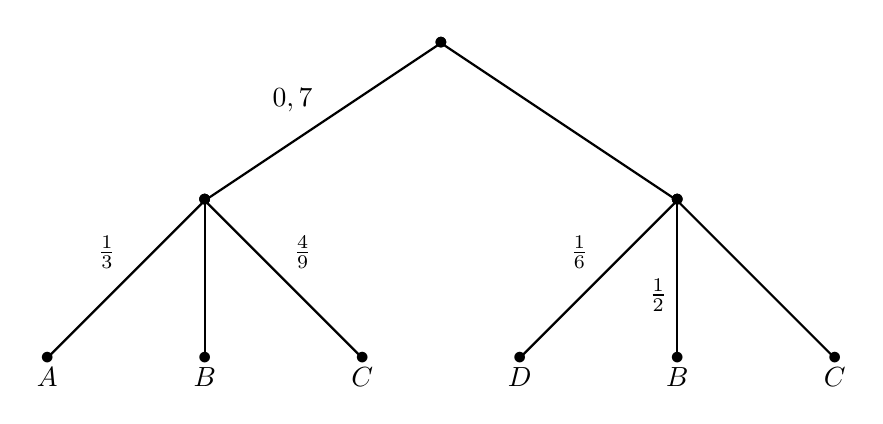
\begin{tikzpicture}
		% depth 1
		\draw[-, thick, black] (0,0) node {$\bullet$} -- (3,-2) node[midway, above right] {};
		\draw[-, thick, black] (0,0) node {$\bullet$} -- (-3,-2) node[midway, above left] {$0,7$};
		% depth 2
		\draw[-, thick, black] (-3,-2) node {$\bullet$} -- (-1,-4) node[midway, above right] {$\frac49$};
		\draw[-, thick, black] (-3,-2) node {$\bullet$} -- (-3,-4);
		\draw[-, thick, black] (-3,-2) node {$\bullet$} -- (-5,-4) node[midway, above left] {$\frac13$};
		
		\draw[-, thick, black] (3,-2) node {$\bullet$} -- (1,-4) node[midway, above left] {$\frac16$};
		\draw[-, thick, black] (3,-2) node {$\bullet$} -- (3,-4) node[pos=.6, left] {$\frac12$};
		\draw[-, thick, black] (3,-2) node {$\bullet$} -- (5,-4);
		
		\draw (1,-4) node {$\bullet$};
		\draw (3,-4) node {$\bullet$};
		\draw (5,-4) node {$\bullet$};
		\draw (1,-4) node[below] {$D$};
		\draw (3,-4) node[below] {$B$};
		\draw (5,-4) node[below] {$C$};
		
		\draw (-1,-4) node {$\bullet$};
		\draw (-3,-4) node {$\bullet$};
		\draw (-5,-4) node {$\bullet$};
		\draw (-1,-4) node[below] {$C$};
		\draw (-3,-4) node[below] {$B$};
		\draw (-5,-4) node[below] {$A$};
	\end{tikzpicture}
	\end{center}
	
	\begin{multicols}{2}
	\begin{enumerate}
		\item Calculer $P(D)$.
		\item Calculer $P(B)$.
		\item Calculer $P(D \cup B)$.
		\item Calculer $P(A\cup C)$.
	\end{enumerate}
	\end{multicols}

}{exe:exe13}{
	La somme des probabilités de chaque sous-branche est toujours $1$. 
	On complète donc l'arbre comme ci-dessous.
	
	\begin{center}
	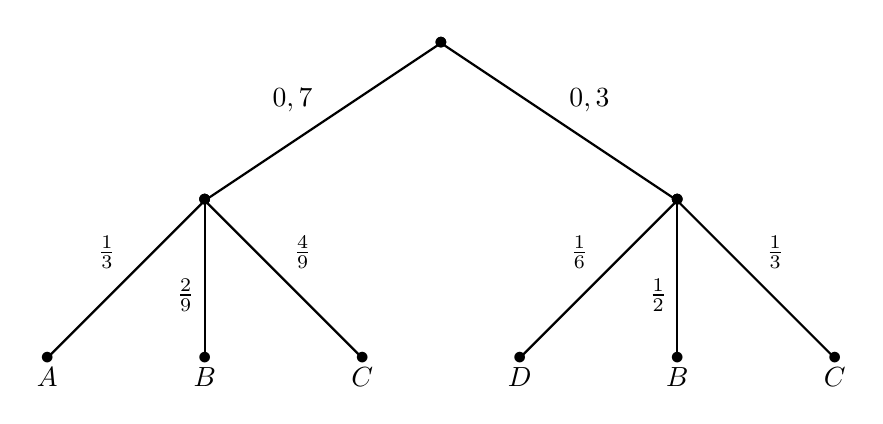
\begin{tikzpicture}
		% depth 1
		\draw[-, thick, black] (0,0) node {$\bullet$} -- (3,-2) node[midway, above right] {$0,3$};
		\draw[-, thick, black] (0,0) node {$\bullet$} -- (-3,-2) node[midway, above left] {$0,7$};
		% depth 2
		\draw[-, thick, black] (-3,-2) node {$\bullet$} -- (-1,-4) node[midway, above right] {$\frac49$};
		\draw[-, thick, black] (-3,-2) node {$\bullet$} -- (-3,-4) node[pos=.6, left] {$\frac29$};
		\draw[-, thick, black] (-3,-2) node {$\bullet$} -- (-5,-4) node[midway, above left] {$\frac13$};
		
		\draw[-, thick, black] (3,-2) node {$\bullet$} -- (1,-4) node[midway, above left] {$\frac16$};
		\draw[-, thick, black] (3,-2) node {$\bullet$} -- (3,-4) node[pos=.6, left] {$\frac12$};
		\draw[-, thick, black] (3,-2) node {$\bullet$} -- (5,-4) node[midway, above right] {$\frac13$};
		
		\draw (1,-4) node {$\bullet$};
		\draw (3,-4) node {$\bullet$};
		\draw (5,-4) node {$\bullet$};
		\draw (1,-4) node[below] {$D$};
		\draw (3,-4) node[below] {$B$};
		\draw (5,-4) node[below] {$C$};
		
		\draw (-1,-4) node {$\bullet$};
		\draw (-3,-4) node {$\bullet$};
		\draw (-5,-4) node {$\bullet$};
		\draw (-1,-4) node[below] {$C$};
		\draw (-3,-4) node[below] {$B$};
		\draw (-5,-4) node[below] {$A$};
	\end{tikzpicture}
	\end{center}
	
	\begin{enumerate}
		\item 
			\begin{align*}
				P(D) &= 0,3 \times \frac16 \\ &= \frac{0,3}{6} \\ &= \frac{3}{60} = \frac1{20}
			\end{align*}
		\item 
			\begin{align*}
				P(B) &= 0,7 \times \frac29 + 0,3 \times \frac12 \\
					&= \frac{1,4}9 + \frac{0,3}2 \\
					&= \frac{14}{90} + \frac3{20} \\
					&= \frac{28}{180} + \frac{27}{180} \\
					&= \frac{55}{180} = \frac{11}{36}
			\end{align*}
		\item 
			Comme $D$ et $B$ sont deux issues distinctes de l'univers, on a
			\begin{align*}
				P(D \cup B) &= P(D) + P(B) \\ &= \frac1{20} + \frac{11}{36}, \\
				&= \frac{18}{360} + \frac{110}{360}, \\
				&= \frac{128}{360} = \frac{64}{180} = \frac{32}{90} = \frac{16}{45}.
			\end{align*}
		\item On peut soit procéder comme ci-dessus, ou alors utiliser le fait que
			\[ P(A\cup C) = P(A) + P(C) = 1 - \left( P(D) + P(B) \right) = 1 - P(D \cup B), \]
		et donc
			\[ P(A\cup C) = 1 - \frac{16}{45} = \frac{29}{45}. \]
	\end{enumerate}
}

\exe{, difficulty=1}{
	On lance 3 fois de suite une pièce de monnaie bien équilibrée.
	Les lancers sont indépendants.
	On note par $P$ (pile) ou $F$ (face) le résultat de chaque lancer.
	Donner $\Omega$, l'univers de l'expérience, et $|\Omega|$ son cardinal.
	
	Calculer la probabilité des événements suivants.
		\begin{multicols}{2}
		\begin{enumerate}
			\item Obtenir $3$ fois face.
			\item Le deuxième lancer donne pile.
			\columnbreak
			\item \mbox{Le troisième lancer est différent du premier.}
			\item On obtient au moins une fois pile.
		\end{enumerate}
		\end{multicols}
}{exe:PF3}{
	Comme les lancers sont distingués, il y a $8$ issues.
		\[ \Omega = \bigset{ FFF ; FFP ; FPF ; FPP ; PFF ; PFP ; PPF ; PPP } \]
	Le cardinal de l'univers est $|\Omega| = 8$.
	On aurait pû aussi noter les issues avec des parenthèses, par exemple $(F;P;F)$, mais pas avec des accolades $\{ \cdot \}$ !
	\begin{enumerate}
		\item
		Les probabilités se multiplient, on a donc $P(FFF) = \frac12 \times \frac12 \times \frac12 = \left( \frac12 \right)^3 = \frac18$.
		En fait, nous sommes en situation d'équiprobabilité, et $|\Omega| = 8$.
		\item 
		Les lancers sont indépendants (le résultat des précédents n'influe en rien celui des prochains), donc la probabilité que le deuxième donne pile est $\frac12$.
		On aurait également pu sommer la probabilité des événements concernés :
			\[ P(FPF) + P(PPF) +  P(FPP) + P(PPP) = \frac48 = \frac12. \]
		\item
		Il y a quatre issues qui correspondent à cet événement. 
			\[ P(PFF) + P(PPF) + P(FFP) + P(FPP) = \frac48 = \frac12. \]
		On aurait pû tout aussi bien supprimer le deuxième lancer, car il n'a aucune influence sur les autres --- cela donne le même résultat.
		\item 
		Lorsqu'on étudie un événement de la forme « au moins [\dots] », il est toujours utile de passer par le complémentaire.
		L'événement complémentaire est « on obtient trois fois face », dont la probabilité est $P(FFF) = \frac18.$
		La probabilité recherché est donc $1-\frac18 = \frac78$.
		
		On aurait également pû énumérer les issues de l'événement et sommer leur probabilité. 
		Seul l'événement $FFF$ n'apparaît alors pas dans cette somme qui vaut $\frac78$.
	\end{enumerate}
}

\newpage



\exe{, difficulty=1}{
	On lance D6 équilibré puis on regarde le numéro de la face du dessus.
	\begin{enumerate}[label=$\bullet$]
		\item Si le numéro obtenu est 1 ou 2, on extrait au hasard une boule dans l'urne A qui contient 3 boules noires, 4 boules blanches et 3 boules rouges
		\item Sinon, on extrait une boule dans l'urne B qui contient 3 boules noires et 2 boules blanches.
	\end{enumerate}
	
	\begin{enumerate}
		\item
		Déduire de l'énoncé les probabilités suivantes. Des fractions irréductibles sont attendues.
		\begin{enumerate}
			\item
			La probabilité de tirer dans l'urne A.
			\item
			La probabilité de tirer une boule blanche lorsque l'on tire dans l'urne A.
			\item
			La probabilité de tirer une boule rouge lorsque l'on tire dans l'urne A.
			\item
			La probabilité de tirer une boule noire lorsque l'on tire dans l'urne B.
		\end{enumerate}
		\item
		Représenter la situation par un arbre de probabilité.
		\item
		\begin{enumerate}
			\item
			Déterminer la probabilité qu'on tire dans l'urne A et qu'on y tire une boule noire.
			\item
			Vérifier que la probabilité de tirer une boule noire est égale à 50\%.
		\end{enumerate}
	\end{enumerate}
}{exe:arbre}{
	On ajoute les probabilités de chacun des événements sur les branches associées.
	Par exemple, de la racine, pour atteindre l'embranchement « obtenir 1 ou 2 », il y a 1 chance sur 3.
	On ajoute donc un $\frac13$ sur la branche qui mène à cet événement, est un $\frac23$ sur l'autre.
	
	En sachant qu'on ait obtenu un nombre qui n'est ni 1 ni 2, on tire une boule dans la deuxième urne  qui contient 3 boules noires et 2 boules blanches.
	La probabilité d'obtenir une boule blanche est donc $\frac25$, et celle d'obtenir une boule noire est $\frac35$.
	En notant toutes les probabilités ainsi calculées, on obtient l'arbre de probabilité suivant.
	
	\begin{center}
	\begin{tikzpicture}
		% depth 1
		\foreach \i in {-3, 3}
		\draw[-, thick, black] (0,0) node {$\bullet$} -- (\i,-2);
		% depth 2
		\foreach \i in {-3} \foreach \j in {-2, 0, 2}
			\draw[-, thick, black] (\i,-2) node {$\bullet$} -- (\i+\j,-4) node {$\bullet$};
			
		\foreach \i in {+3} \foreach \j in {-1, 1}
			\draw[-, thick, black] (\i,-2) node {$\bullet$} -- (\i+\j,-4) node {$\bullet$};
			
		\draw (0,0) node[above] {Départ};
		\draw (-3,-2) node[left] {urne A};
		\draw (3,-2) node[right] {urne B};
		\draw (4,-4) node[below] {B};
		\draw (2,-4) node[below] {N};
		\draw (-1,-4) node[below] {B};
		\draw (-3,-4) node[below] {N};
		\draw (-5,-4) node[below] {R};
		
		\draw (1.5, -1) node[above right] {$\dfrac23$};
		\draw (-1.5, -1) node[above left] {$\dfrac13$};
		
		\draw (3.5, -3.25) node[above right] {$\frac25$};
		\draw (2.5, -3.25) node[above left] {$\frac35$};
		
		\draw (-2, -3.25) node[above right] {$\frac25$};
		\draw (-3, -3.25) node[left] {$\frac3{10}$};
		\draw (-4, -3.25) node[above left] {$\frac3{10}$};
	\end{tikzpicture}
	\end{center}
	La probabilité d'un chemin racine-feuille est le produit des probabilités rencontrées en le parcourant.
	En outre, deux tels chemins correspondent à des événements disjoints.
	On calcule donc
		\[ P(N) = \dfrac23 \cdot \dfrac35 + \dfrac13 \cdot \dfrac3{10} = \dfrac12. \]
}



%\exe{}{
%	On tire un boule dans une urne contenant $2$ boules rouges et $4$ boules vertes.
%	\begin{enumerate}[label=$\bullet$]
%		\item Si la boule tirée est verte, on la met de côté et on retire une nouvelle boule
%		\item Si la boule tirée est rouge, on la remet dans l'urne et on retire une nouvelle boule
%	\end{enumerate}
%	On distingue les quatre événements suivants :
%		\begin{multicols}{2}
%		\begin{enumerate}[label=]
%			\item v : « la première boule tirée est verte »
%			\item r : « la première boule tirée est rouge »
%			\item V : « la deuxième boule tirée est verte »
%			\item R : « la deuxième boule tirée est rouge »
%		\end{enumerate}
%		\end{multicols}
%	\begin{center}
%	\begin{tikzpicture}
%		% depth 1
%		\foreach \i in {-3, 3}
%		\draw[-, thick, black] (0,0) node {$\bullet$} -- (\i,-2);
%		% depth 2
%		\foreach \i in {-3, 3} \foreach \j in {-1, 1}
%			\draw[-, thick, black] (\i,-2) node {$\bullet$} -- (\i+\j,-4) node {$\bullet$};
%			
%		\draw (-3,-2) node[above left] {v};
%		\draw (3,-2) node[above right] {r};
%			
%		\draw (-4,-4) node[below] {V};
%		\draw (2,-4) node[below] {V};
%		\draw (-2,-4) node[below] {R};
%		\draw (4,-4) node[below] {R};
%	\end{tikzpicture}
%	\end{center}
%	Compléter l'arbre, et calculer $P(V)$ et $P(R)$.
%}{exe:exe12}{
%	\, \\
%	\begin{center}
%	\begin{tikzpicture}
%		% depth 1
%		\foreach \i in {-3, 3}
%		\draw[-, thick, black] (0,0) node {$\bullet$} -- (\i,-2);
%		% depth 2
%		\foreach \i in {-3, 3} \foreach \j in {-1, 1}
%			\draw[-, thick, black] (\i,-2) node {$\bullet$} -- (\i+\j,-4) node {$\bullet$};
%			
%		\draw (-3,-2) node[above left] {v};
%		\draw (3,-2) node[above right] {r};
%			
%		\draw (-4,-4) node[below] {V};
%		\draw (2,-4) node[below] {V};
%		\draw (-2,-4) node[below] {R};
%		\draw (4,-4) node[below] {R};
%		
%		% sols
%		\draw (1.5,-.5) node {$\frac13$};
%		\draw (-1.5,-.5) node {$\frac23$};
%		
%		\draw (4,-3) node {$\frac13$};
%		\draw (2,-3) node {$\frac23$};
%		
%		\draw (-2,-3) node {$\frac25$};
%		\draw (-4,-3) node {$\frac35$};
%	\end{tikzpicture}
%	\end{center}
%	La probabilité d'une issue est la somme des probabilités de chacun des chemins racine-feuille.
%	Pour obtenir la probabilité d'un chemin racine-feuille, on multiplie les probabilités rencontrées en le parcourant.
%	
%		\begin{align*}
%			P(V) &= \frac23 \times \frac35 + \frac13 \times \frac23 \\
%				&= \frac25 + \frac29 \\
%				&= \frac{18 + 10}{5 \times 9} = \frac{28}{45}
%		\end{align*}
%	
%		\begin{align*}
%			P(R) &= \frac23 \times \frac25 + \frac13 \times \frac13 \\
%				&= \frac4{15} + \frac19 \\
%				&= \frac{36 + 15}{15 \times 9} = \frac{51}{135} = \frac{17}{45}
%		\end{align*}
%		
%		On aurait aussi pû utiliser le fait que $P(R) = 1 - P(V)$ pour ne pas augmenter la probabilité de faire une erreur de calcul.
%}


%
%\exe{}{
%	On tire un boule dans une urne contenant 3 boules bleues et 4 boules vertes.
%	\begin{enumerate}[label=$\bullet$]
%		\item Si la boule tirée est verte, on jette un dé équilibré à 3 faces (1 à 3).
%		\item Si la boule tirée est bleue, on jette un dé équilibré à 6 faces (1 à 6).
%	\end{enumerate}
%
%	Créer un arbre de probabilité pour cette situation et répondre aux questions suivantes. Donner les probabilités sous forme de fraction irréductible.
%	\begin{enumerate}
%		\item Quelle est la probabilité d'obtenir un nombre pair ?
%		\item Quelle est la probabilité d'obtenir un multiple de $3$ ?
%		\item Quelle est la probabilité d'obtenir un nombre pair \textbf{ou} un multiple de $3$ ?
%		\item Calculer la probabilité d'obtenir $6$.
%		\item Énoncer le principe d'inclusion-exclusion et le vérifier.
%	\end{enumerate}
%
%}{exe:exe14}{
%	On a l'arbre suivant.
%	
%	\begin{center}
%	\begin{tikzpicture}
%		% depth 1
%		\draw[-, thick, black] (0,0) node {$\bullet$} -- (4,-2) node[midway, above right] {$\frac37$};
%		\draw[-, thick, black] (0,0) node {$\bullet$} -- (-3,-2) node[midway, above left] {$\frac47$};
%		% depth 2
%		% gauche -> droite
%		% verte
%		\draw[-, thick, black] (-3,-2) node {$\bullet$} -- (-2,-4) node[midway, above right] {$\frac13$};
%		\draw[-, thick, black] (-3,-2) node {$\bullet$} -- (-3,-4) node[pos=.6, left] {$\frac13$};
%		\draw[-, thick, black] (-3,-2) node {$\bullet$} -- (-4,-4) node[midway, above left] {$\frac13$};
%		
%		\draw (-4,-4) node {$\bullet$};
%		\draw (-3,-4) node {$\bullet$};
%		\draw (-2,-4) node {$\bullet$};
%		\draw (-4,-4) node[below] {$1$};
%		\draw (-3,-4) node[below] {$2$};
%		\draw (-2,-4) node[below] {$3$};
%		
%		% bleue
%		\draw[-, thick, black] (4,-2) node {$\bullet$} -- (0,-4) node[midway, above left] {$\frac16$};
%		\draw[-, thick, black] (4,-2) node {$\bullet$} -- (1.5,-4) node[pos=.6, left] {$\frac16$};
%		\draw[-, thick, black] (4,-2) node {$\bullet$} -- (3,-4) node[midway, right] {$\frac16$};
%		\draw[-, thick, black] (4,-2) node {$\bullet$} -- (4.5,-4) node[midway, left] {$\frac16$};
%		\draw[-, thick, black] (4,-2) node {$\bullet$} -- (6,-4) node[midway, right] {$\frac16$};
%		\draw[-, thick, black] (4,-2) node {$\bullet$} -- (7.5,-4) node[midway, above right] {$\frac16$};
%		
%		\draw (0,-4) node {$\bullet$};
%		\draw (1.5,-4) node {$\bullet$};
%		\draw (3,-4) node {$\bullet$};
%		\draw (4.5,-4) node {$\bullet$};
%		\draw (6,-4) node {$\bullet$};
%		\draw (7.5,-4) node {$\bullet$};
%		\draw (0,-4) node[below] {$1$};
%		\draw (1.5,-4) node[below] {$2$};
%		\draw (3,-4) node[below] {$3$};
%		\draw (4.5,-4) node[below] {$4$};
%		\draw (6,-4) node[below] {$5$};
%		\draw (7.5,-4) node[below] {$6$};
%		
%	\end{tikzpicture}
%	\end{center}
%	
%	\begin{enumerate}
%		\item
%			\begin{align*}
%				P(\text{« nombre pair »}) &= P(2) + P(4) + P(6) \\
%					&= \left( \frac47 \times \frac13 + \frac37\times\frac16 \right) + \left( \frac37 \times \frac16 \right) + \left( \frac37 \times \frac16 \right) \\
%					&= \frac4{21} + \frac1{14} + \frac1{14} + \frac1{14} \\
%					&= \frac{17}{42}.
%			\end{align*}
%		\item
%			\begin{align*}
%				P(\text{« multiple de $3$ »}) &= P(3) + P(6) \\
%					&= \left( \frac47 \times \frac13 + \frac37\times\frac16 \right) + \left( \frac37 \times \frac16 \right) \\
%					&= \frac4{21} + \frac1{14} + \frac1{14} \\
%					&= \frac13.
%			\end{align*}
%		\item
%			\begin{align*}
%				P(\text{« multiple de $3$ ou de $2$ »}) &= P(2) + P(3) + P(4) + P(6) \\
%					&= \left( \frac47 \times \frac13 + \frac37\times\frac16 \right) + \left( \frac47 \times \frac13 + \frac37\times\frac16 \right) + \left( \frac37 \times \frac16 \right) + \left( \frac37 \times \frac16 \right) \\
%					&= \frac4{21} + \frac1{14} + \frac4{21} + \frac1{14} + \frac1{14} + \frac1{14} \\
%					&= \frac23.
%			\end{align*}
%		\item 
%			\begin{align*}
%				P(6) &=\left( \frac37 \times \frac16 \right) \\
%					&= \frac1{14}.
%			\end{align*}
%		
%		\item
%		On vérifie l'inclusion-exclusion en comparant $P(\text{« multiple de $3$ ou de $2$ »})$ et $P(\text{« multiple de $3$ »}) + P(\text{« multiple de $2$ »}) - P(6)$.
%		D'une part,
%			\[ P(\text{« multiple de $3$ ou de $2$ »}) = \frac23, \]
%		et d'autre part,
%			\begin{align*}
%				P(\text{« multiple de $3$ »}) + P(\text{« multiple de $2$ »}) - P(6) &= \frac13 + \frac{17}{42} - \frac1{14} \\
%				&= \frac{14 + 17 - 3}{42} \\
%				&= \frac{28}{42} = \frac23.
%			\end{align*}
%	\end{enumerate}
%}

\exe{}{
	Dans une urne opaque se trouvent un nombre inconnu de boules rouges, bleues, et vertes.
	On tire aléatoirement une boule de l'urne, on note sa couleur, et on la remet dans l'urne.
	Les résultats sont décrits dans le tableau suivant.
	\begin{center}
	\begin{tabular}{|c|c|c|c|} \hline
		Couleur & Rouge & Bleu & Vert \\ \hline
		Nombre de tirages & 35~040 & 53~468 & 17~982 \\ \hline
		Fréquence & & & \\ \hline
	\end{tabular}
	\end{center}
	
	Compléter le tableau en arrondissant à $10^{-2}$ près, \underline{modéliser la réalité} en définissant un univers et une loi de probabilité, et l'utiliser pour répondre aux questions suivantes.
	\begin{enumerate}
		\item Quelle est la probabilité d'obtenir deux boules rouges en deux tirages ?
		\item Quelle est la probabilité d'obtenir deux boules vertes en trois tirages ?
		\item \calculator{\Large} Quelle est la probabilité d'obtenir au moins une boule bleue en quatre tirages ? 
	\end{enumerate}
}{exe:exe15}{
	Les fréquences sont calculées à $10^{-2}$ près dans le tableau ci-dessous.
	
	
	\begin{center}
	\begin{tabular}{|c|c|c|c|} \hline
		Couleur & Rouge & Bleu & Vert \\ \hline
		Nombre de tirages & 35~040 & 53~468 & 17~982 \\ \hline
		Fréquence & $\color{RED_E} 0,33$  & $\color{RED_E} 0,50$ & $\color{RED_E} 0,16$ \\ \hline
	\end{tabular}
	\end{center}
	
	
	Modélisons la réalité en assignant les probabilités suivantes.
		\begin{align*}
			P(\text{Rouge}) = \frac13 && P(\text{Bleu}) = \frac12 && P(\text{Vert}) = \frac16
		\end{align*}
	On vérifie bien sûr que la somme fasse bien $1$ : $\frac13 + \frac12 + \frac16 = 1$.

	\begin{enumerate}
		\item 
			On crée un arbre binaire de profondeur $2$ à deux événements : $E$ et $\overline{E}$ où
				\begin{center}
					E : « tirer une boule rouge ».
				\end{center}
			On en déduit que
			\[ P(\text{deux boules rouges en deux tirages}) = \frac13 \times \frac13 = \frac19. \]
		\item 
			On crée un arbre binaire de profondeur $3$ à deux événements : $F$ et $\overline{F}$ où
				\begin{center}
					F : « tirer une boule verte ».
				\end{center}
			On lit trois issues pour l'événement : $FF\overline{F}$, $F\overline{F}F$, et $\overline{F}FF$.
			Chaque issue a probabilité $\frac16 \times \frac16 = \frac1{36}$, donc
			\[ P(\text{deux boules vertes en trois tirages}) = 3\times \frac1{36} = \frac1{12}. \]
		\item Quelle est la probabilité d'obtenir au moins une boule bleue en quatre tirages ?
			On crée un arbre binaire de profondeur $4$ à deux événements : $G$ et $\overline{G}$ où
				\begin{center}
					G : « tirer une boule bleue ».
				\end{center}
			On lit une seule issue pour l'événement complémentaire, et donc
			\[ P(\text{aucune boule bleue en quatre tirages}) = \frac12\times\frac12\times\frac12\times\frac12= \frac{1}{16}. \]
			Par conséquent, 
			\[ P(\text{au moins une boule bleue en quatre tirages}) =1- \frac{1}{16} = \frac{15}{16} = 0,9375. \]
	\end{enumerate}
}

\exe{}{
	On lance un grand nombre de fois un D$6$, dé à $6$ faces.
	Les résultats sont décrits dans le tableau suivant.
	\begin{center}
	\begin{tabular}{|c|c|c|c|c|c|c|} \hline
		Face & 1 & 2 & 3 & 4 & 5 & 6 \\ \hline
		Nombre de tirages & $29~309$ & $43~498$ & $14~465$ & $22~116$ & $29~212$ & $7~281$ \\ \hline
		Fréquence & &&&&&\\ \hline
	\end{tabular}
	\end{center}
	
	Compléter le tableau en arrondissant à $10^{-2}$ près, \underline{modéliser la réalité} en définissant un univers et une loi de probabilité, et l'utiliser pour répondre aux questions suivantes.
	\begin{enumerate}
		\item Quelle est la probabilité d'obtenir un nombre pair ?
		\item Quelle est la probabilité d'obtenir deux 6 en deux lancers consécutifs ?
		\item\calculator{\Large} Quelle est la probabilité d'obtenir au moins un 6 après quatre lancers ?
	\end{enumerate}
}{exe:exe16}{
	Les fréquences sont calculées à $10^{-2}$ près dans le tableau ci-dessous.
	
	\begin{center}
	\begin{tabular}{|c|c|c|c|c|c|c|} \hline
		Face & 1 & 2 & 3 & 4 & 5 & 6 \\ \hline
		Nombre de tirages & $29~309$ & $43~498$ & $14~465$ & $22~116$ & $29~212$ & $7~281$ \\ \hline
		Fréquence &  $\color{RED_E} 0,2$  &  $\color{RED_E} 0,3$  &  $\color{RED_E} 0,1$  &  $\color{RED_E} 0,15$  &  $\color{RED_E} 0,2$  &  $\color{RED_E} 0,05$  \\ \hline
	\end{tabular}
	\end{center}
	
	Modélisons la réalité en assignant les probabilités suivantes.
		\begin{align*}
			P(1) = \frac15 && P(2) = \frac3{10} && P(3) = \frac1{10} && P(4) = \frac3{20} && P(5) = \frac15 && P(6) = \frac1{20}
		\end{align*}
	On s'assure bien que la somme soit $1$ : 
		\[ \frac15 + \frac3{10} + \frac1{10} + \frac3{20} + \frac15 + \frac1{20} = \frac{4+6+2+3+4+1}{20} = 1. \]
	
	\begin{enumerate}
		\item 
			\begin{align*}
				P(\text{« obtenir un nombre pair »}) &= P(2) + P(4) + P(6) \\
				&= 0,3 + 0,15 + 0,05 \\
				&= 0,5 = \frac12.
			\end{align*}
		\item
			On crée un arbre binaire de profondeur $2$ à deux événements : $E$ et $\overline{E}$ où
				\begin{center}
					E : « obtenir $6$ ».
				\end{center}
			On en déduit que
			\[ P(\text{deux $6$ en deux lancers}) = 0,05 \times 0,05 = \left(\frac1{20}\right)^2 = \frac1{400} = 0,0025. \]
		\item
			On complète l'arbre binaire de la question précédente pour qu'il atteigne une profondeur $4$.
			L'événement complémentaire correspond à une unique issue, de probabilité
				\[ P(\text{aucun $6$ en $4$ lancers}) = 0.95^4 = \left(\frac{19}{20}\right)^4 = \frac{19^4}{20^4} = \frac{130321}{160000} \approx 0,81. \]
			On conclut donc que
				\[ P(\text{au moins un $6$ en $4$ lancers}) = 1-0.95^4 \approx 0,19. \]
				
	\end{enumerate}
}


\exe{, difficulty=2}{
	On lance un D6 pipé avant de noter le numéro de la face du dessus.
	Les probabilités de chacunes des issues vérifient
		\[ P(1) = 2 P(2) = P(3) = 2 P(4) = P(5) = 2P(6). \]
	Calculer $P($« le résultat est divisible par $3$ »$)$.
}{exe:dur1}{
	Posons $p=P(2) \in [0;1]$ et exprimons chaque probabilité en fonction de $p$.
		\begin{align*}
			P(1) = 2p && P(2) = p && P(3) = 2p && P(4) = p && P(5) = 2p && P(6) = p.
		\end{align*}
	La relation $P(\Omega) = 1$ nous donne l'équation suivante à résoudre pour $p$.
		\begin{align*}
			P(1) + P(2) + P(3) + P(4) + P(5) + P (6) &= 1 \\
			2p + p + 2p + p + 2p + p &= 1 \\
			9p &= 1 \\
			p &= \frac19
		\end{align*}
	On en déduit le tableau de probabilités suivant.
	\begin{center}
	\begin{tabular}{|c|c|c|c|c|c|c|} \hline
		Résultat & 1 & 2 & 3 & 4 & 5 & 6 \\ \hline
		Probabilité & $\frac29$ & $\frac19$ & $\frac29$ & $\frac19$ & $\frac29$ & $\frac19$ \\ \hline
	\end{tabular}
	\end{center}
	Et on conclut que $P($« le résultat est divisible par $3$ »$) = P(3) + P(6) = \frac29 + \frac19 = \frac13.$
}

\exe{, difficulty=1}{
	L'univers associé à une expérience aléatoire est $\{ a, b, c\}$.
	La loi de probabilité $P$ vérifie $P(a) = t^2$, $P(b) = -t$, et $P(c) = \frac14$, pour un réel $t \in \R$.
	
	Développer le carré $\left(t-\frac12\right)^2$ et déterminer $t$.
}{exe:dur2}{
	On développe le carré à l'aide de l'identité remarquable
		\[ (a-b)^2 = a^2 + b^2 - 2ab, \]
	où, ici, on a $a=t$ et $b=\frac12.$
		\begin{align*}
			\left(t-\frac12\right)^2 &= t^2 + \left(\frac12\right)^2 - 2 \cdot t \cdot \frac12 \\
									&= t^2 + \frac14 - t
		\end{align*}
	On cherche désormais le $t\in\R$ pour lequel $P$ est une loi de probabilité. 
	Un loi vérifie les deux propriétés suivantes :
		\begin{itemize}
			\item $P(\omega) \in [0;1]$ pour chaque issue $\omega \in \Omega$ ; et
			\item $P(\Omega) = 1$.
		\end{itemize}
	La deuxième identité donne donc
		\begin{align*}
			P(a) + P(b) + P(c) = 1 && \iff && t^2 - t + \frac14 = 1.
		\end{align*}
	Le carré développé nous permet d'écrire
		\[ \left(t-\frac12\right)^2 = 1, \]
	et donc
		\[ \left|t-\frac12\right| = \sqrt{1} = 1, \]
	en utilisant le fait que $\sqrt{x^2} = |x|.$
	L'expression à l'intérieur de la valeur absolue est donc soit $+1$, soit $-1$, et on a donc deux alternatives :
		\begin{align*}
			t-\frac12 = 1 && \text{ ou } && t - \frac12 = -1 \\
			t = \frac32 && \text{ ou } && t = -\frac12.
		\end{align*}
	%Pour s'entraîner à ce genre de résolution, voir la feuille d'exercices Fonctions 3.
	
	Comme les probabilités sont des nombres entre $0$ et $1$, on peut écarter la première solution car $P(a) = t^2$ serait strictement supérieur à $1$, et $P(b) = -t$, serait strictement négatif.
	Il ne reste donc que $t = -\frac12$, qui donne le tableau de probabilités suivant.
	\begin{center}
	\begin{tabular}{|c|c|c|c|} \hline
		Issue & $a$ & $b$ & $c$ \\ \hline
		Probabilité & $\frac14$ & $\frac12$ & $\frac14$ \\ \hline
	\end{tabular}
	\end{center}
}


\exe{, difficulty=1}{
	Dessiner des diagrammes de Venn pour motiver les relations suivantes.
		\begin{align*}
			\overline{A\cup B} = \overline{A} \cap \overline{B}, && \text{et} && \overline{A \cap B} = \overline{A} \cup \overline{B}.
		\end{align*}

}{exe:Venn-new}{
	En classe.
}



\exe{, difficulty=1}{
	On lance deux D6 équilibrés, dés à 6 faces l'un après l'autre. Les deux dés sont distinguables car de couleurs différentes.
	\begin{enumerate}
		\item Donner l'univers $\Omega$ et son cardinal $|\Omega|$. Est-ce une situation d'équiprobabilité ?
		\item Quelle est la probabilité d'obtenir un double 6 ?
		\item\calculator{\Large} Quelle est la probabilité qu'après 10 tels lancers, on obtienne au moins une fois un \mbox{double 6 ?}
	\end{enumerate}
}{exe:dur5}{
	\begin{enumerate}
		\item Donner l'univers $\Omega$ et son cardinal $|\Omega|$. Est-ce une situation d'équiprobabilité ?
		L'univers est formé par tous les couples $(a ;b)$ de résultats.
		On utilise des parenthèses ici car on distingue le premier du deuxième lancer.
			\[ \Omega = \Bigset{ (a ; b) \text{ où } a, b \in \bigset{ 1 ; 2 ; 3 ; 4 ;5 ; 6 } }, \]
		de cardinal $|\Omega| = 6 \times 6 = 36$.
		
		La situation est bien d'équiprobabilité car il y a 36 issues et chacune admet comme probabilité $\frac16 \times \frac16 = \frac1{36}$, car les dés sont bien équilibrés.
		
		\item 
		La probabilité de l'issue $(6;6)$ est $\frac1{36}$ par équiprobabilité.
		
		\item
		Lorsqu'on étudie un événement de la forme « au moins [\dots] », il est toujours utile de passer par le complémentaire.
		L'événement complémentaire est « obtenir aucun double 6 », dont la probabilité est
			\[ \left( \frac{35}{36} \right)^{10} \approx 0,75. \]
		En effet, on peut construire un arbre réduit à deux événements  : « double 6 » (probabilité $\frac1{36}$) et « pas double 6 » (probabilité $\frac{35}{36}$), de profondeur $10$.
		La feuille qui correspond à « obtenir aucun double 6 » est obtenue en tournant vers « pas double 6 » dix fois dans l'arbre.
		
		La probabilité de l'événement « on obtient aucun double 6 » est donc
			\[ \left( \frac{35}{36} \right)^{10} \approx 0,75. \]
		On conclut en faisant $1-0,75 = 0,25$, probabilité approximative qu'au moins un des 10 lancers donne un double 6.
	\end{enumerate}


}



\exe{, difficulty=1}{
	On lance deux D$6$ équilibrés, dés à $6$ faces, au même moment. Les deux dés sont absolument identiques.
	\begin{enumerate}
		\item Donner l'univers $\Omega$ et son cardinal $|\Omega|$. 
		\item Quelle est la probabilité d'obtenir un double $6$ ? Est-ce une situation d'équiprobabilité ?
		\item Quelle est la probabilité d'obtenir deux résultats différents ?
	\end{enumerate}
}{exe:dur9}{	
	\begin{enumerate}
		\item
		L'ordre des résultats n'importe pas car les dés sont identiques et les jets effectués au même moment.		
		On a donc 
		\begin{align*}
			\Omega &= \Bigset{ \{a ; b \} \text{ où } a, b \in \bigset{ 1 ; 2 ; 3 ;4 ;5 ;6} } \\
					&= \left\{
						\begin{aligned}
						&\{1 ; 1\}, \{1 ; 2\}, \{1 ; 3\}, \{1 ; 4\}, \{1 ; 5\}, \{1 ; 6\}, \\
						&\{2 ; 2\}, \{2 ; 3\},\{2 ; 4\}, \{2 ; 5\}, \{2 ; 6\}, \\
						& \{3 ; 3\}, \{3 ; 4\}, \{3 ; 5\}, \{3 ; 6\}, \\
						& \{4 ; 4\}, \{4 ; 5\}, \{4 ; 6\}, \\
						& \{5 ; 5\}, \{5 ; 6\}, \\
						& \{6 ; 6\}
						\end{aligned}
						\right\}
		\end{align*}
		On compte $|\Omega| = 6 + 5 + 4 + 3 + 2 + 1 = 21$.
		
		Un autre façon de compter sans énumérer est la suivante : chaque paire de résultats distincts est comptée deux fois au lieu d'une. 
		Il y a $6$ paires de résultats identiques, donc $36-6 = 30$ paires de résultats distincts.
		Par conséquent, $|\Omega| = \frac{30}2 + 6 = 21$.
		
		\item Il n'y a qu'une seule façon d'obtenir un double $6$ : que les deux dés résultent en un $6$.
		Ainsi $P\bigl( \{6 ; 6\} \bigr) = \frac16 \times \frac16 = \frac1{36}$.
		
		Pour comprendre la probabilité de chaque événement, il est possible de différencier les deux dés (par exemple en leur assignant une couleur), et de regrouper les issues qui donnent le même résultat lorsque les dés sont identiques.
		Par exemple, « obtenir 5 puis obtenir 6 » et « obtenir 6 puis obtenir 5 » sont deux issues différentes équiprobables si les dés sont différentiables, mais pas si les dés sont identiques et les lancers simultanés.
		La situation n'est donc pas une situation d'équiprobabilité car toutes les issues n'ont pas la même probabilité d'arriver.
		Par exemple,
			\[ P\bigl( \{2 ; 2\} \bigr) = \frac1{36} \qquad \et \qquad P\bigl(\{5 ; 6\}\bigr) = \frac2{36} = \frac1{18}, \]
		car il y a deux façons d'obtenir l'issue $\{5 ; 6\}$.
		\item 
		Pour calculer la probabilité d'obtenir deux résultats identiques, on additionne 
			\[ P\bigl( \{1 ; 1\} \bigr) + P\bigl( \{2 ; 2\} \bigr)+ P\bigl( \{3 ; 3\} \bigr)+ P\bigl( \{4 ; 4\} \bigr)+ P\bigl( \{5 ; 5\} \bigr)+ P\bigl( \{6 ; 6\} \bigr) = \frac{6}{36} = \frac16. \]
		Par conséquent, la probabilité d'obtenir deux résultats différents est égale à
			$1 - \frac16 = \frac56. $
	\end{enumerate}
}


\subsection*{Approfondissements}



\exe{, difficulty=2}{
	On choisit deux nombres $x$ et $y$ aléatoirement et uniformément entre 0 et 1, et on considère la distance $d$ du point $(x;y)$ à l'origine.
	On souhaite calculer la probabilité $p$ de l'événement « la distance $d$ est inférieure à 1 ».
	
	\begin{enumerate}
		\item
		Faire un dessin de la situation et justifier que $p = \frac{\pi}4$.
		\item
		Créer un protocole pour approximer la valeur de $\pi$ en admettant qu'on puisse choisir un nombre uniformément entre 0 et 1.
	\end{enumerate}
	En important le module Python NumPy à l'aide de \texttt{import numpy}, il est possible de générer un nombre aléatoirement\footnotemark entre 0 et 1 grâce à \texttt{numpy.random.rand()}.
	\begin{enumerate}[resume]
		\item
		En utilisant $N=10^7$ points $(x;y)$ générés aléatoirement, estimer la valeur de $\pi$ à $10^{-3}$ près après avoir implémenté le protocole décrit.
	\end{enumerate}
}{exe:app2}{
	À rendre pour possibilité de points bonus à la prochaine évaluation.
	Ni correction ni points ne seront attribués à un travail suspect ou ne démontrant pas une bonne compréhension de l'exercice.


	Cet exercice traite de la \emph{méthode de Monte Carlo} qui se base sur la loi faible des grands nombres : la fréquence s'approche de la probabilité lorsque le nombre d'échantillons augmente.
	
	Une ébauche d'algorithme est disponible ci-dessous.
	
	En 1943, pendant la Seconde Guerre Mondiale, Robert Oppenheimer recrute Nicholas Metropolis à Los Alamos afin qu'il aide à développer un modèle pour décrire l'état des matériaux physiques.
	Metropolis étant, avec ses collègues Richard Feynman et John von Neumann, fatigué de la lenteur des calculettes de l'époque, il dirigea en 1948 le premier super-ordinateur programmable : MANIAC.
	L'algorithme Metropolis puis Metropolis-Hastings, parent de la méthode de Monte Carlo et publié après la fin de la guerre, donna naissance à la \emph{thermodynamique statistique} permettant d'étudier des systèmes à et hors équilibre thermodynamique.
	Le modèle d'Ising est un exemple classique d'étude ferromagnétique avec comme paramètre la température du matériau.
	
	Voir \emph{A History of the Metropolis-Hastings Algorithm} de David B. Hitchcock pour une exposition plus complète.

	
	\python{MonteCarlo}
}

\footnotetext{Pas \emph{exactement} aléatoirement : la plupart des nombres ne sont pas représentables par un ordinateur.}


%\exe{, difficulty=2}{
%	On mélange un jeu classique de $52$ cartes puis on retourne les cartes une à une en les prenant successivement du haut du paquet.
%	Quelle est la probabilité que l'as de trèfle soit le premier as retourné ?
%
%	On ajoute une carte joker au paquet avant de le remélanger et de retourner encore une fois les cartes une à une.
%	Quelle est la probabilité que le joker apparaisse après exactement un as, et avant les trois autres ?
%}{exe:app1}{
%
%}

\exe{, difficulty=3}{
	On lance une pièce lestée dont la probabilité d'obtenir « pile » est $p$ et « face » est $q$.
	Notons $X$ le nombre de « face » obtenus avant le premier « pile ».
	\begin{multicols}{2}
	\begin{enumerate}
		\item
		Écrire $p$ en fonction de $q$.
		\item
		%Vérifier que la probabilité que $X$ vale 0 est $p$.
		Vérifier que $P(X=0) = p$.
		\item
		Donner la probabilité que $X$ soit égale à 1.
		\item 
		%Vérifier que la probabilité que $X$ vale 2 est $q^2p$.
		Vérifier que $P(X=2) = q^2p$.
	\end{enumerate}
	\end{multicols}
	\begin{enumerate}[start=5]
		\item
		En déduire l'égalité suivante, la somme étant infinie.
			\begin{align*}
				p\cdot \bigl(1 + q + q^2 + q^3 + \hdots\bigr) = 1 && \iff && 1 + q + q^2 + q^3 + \hdots = \frac1{1-q}
			\end{align*}
		\item
		Quelles identités obtient-on si $q = \frac1{10}$ ? Et si $q = \frac12$ ?
	\end{enumerate}
}{exe:app3}{
	À rendre pour possibilité de points bonus à la prochaine évaluation.
	Ni correction ni points ne seront attribués à un travail suspect ou ne démontrant pas une bonne compréhension de l'exercice.

	Cet exercice est une introduction à la \emph{loi géométrique} qui enregistre le premier succès après répétition d'une même expérience.
	
	Il traite également des sommes infinies dont on donnera le sens suivant.
	D'après un précédent exercice d'approfondissement, la somme finie vaut
		\[ 1 + q + q^2 + \cdots + q^{N-1} = \frac{1-q^N}{1-q}. \]
	Or, si $q<1$, comme c'est le cas pour une probabilité, alors $q^N$ devient très très très petit lorsque $N$ grandit (prendre par exemple $q=0,1$ et $N=10^{10^{10}}$).
	Lorsque $N$ tend vers l'infini (lire : devient très très grand), $1-q^N$ tend vers 1 (lire : très très proche de 1), ce qui permet de justifier proprement de l'égalité obtenue.
}

%%%%%%%%%%%

\newpage
\fancyhead[C]{\textbf{Solutions}}
\shipoutAnswer

\end{document}
